\documentclass{article}
\usepackage{pdfpages}
\usepackage{float}
\usepackage{enumerate}
\usepackage{amsmath}
\usepackage{amssymb}
\usepackage{graphicx}
\usepackage{url}
\usepackage{subfig}
\usepackage[margin=0.25in]{geometry}

\begin{document}

\section{Anti-Aliasing}

\begin{figure}[H]
    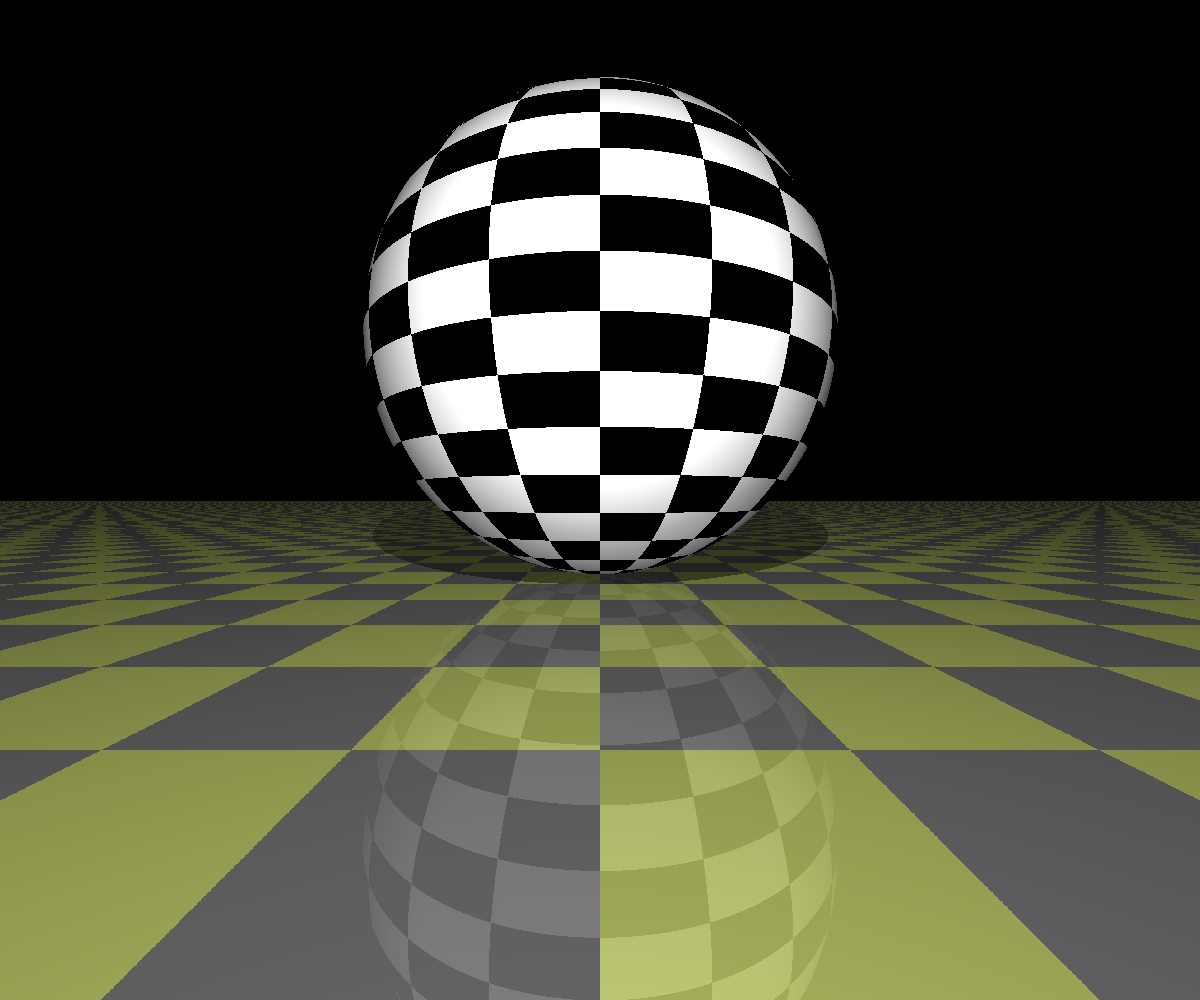
\includegraphics[width=\textwidth]{./examples/AntiAliasingComparison/Scene_noAntiAliasing.png}
    \caption{No anti-aliasing.}
\end{figure}

\begin{figure}[H]
    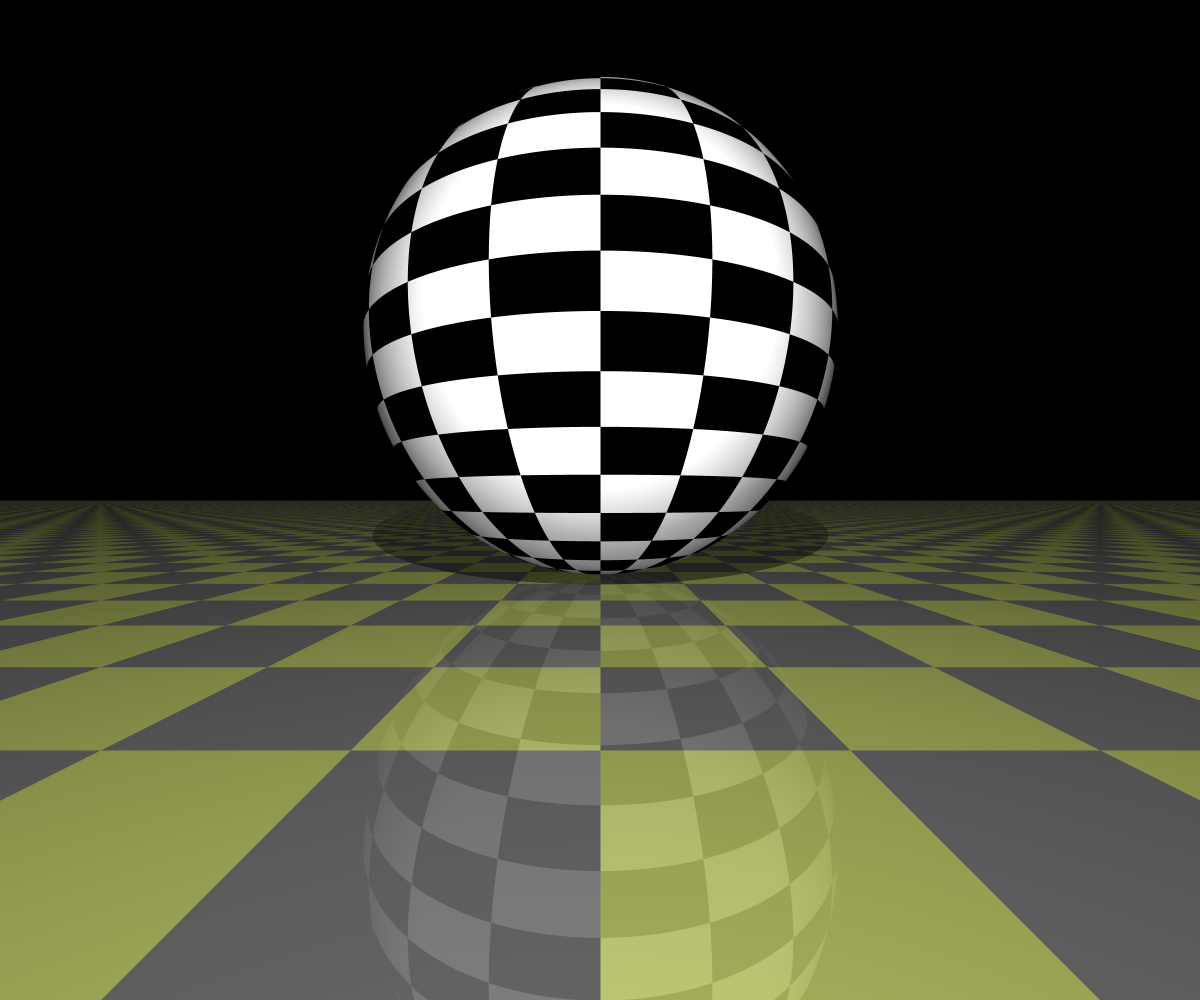
\includegraphics[width=\textwidth]{./examples/AntiAliasingComparison/Scene_regular64.png}
    \caption{64x AA using regular sampling.}
\end{figure}

\begin{figure}[H]
    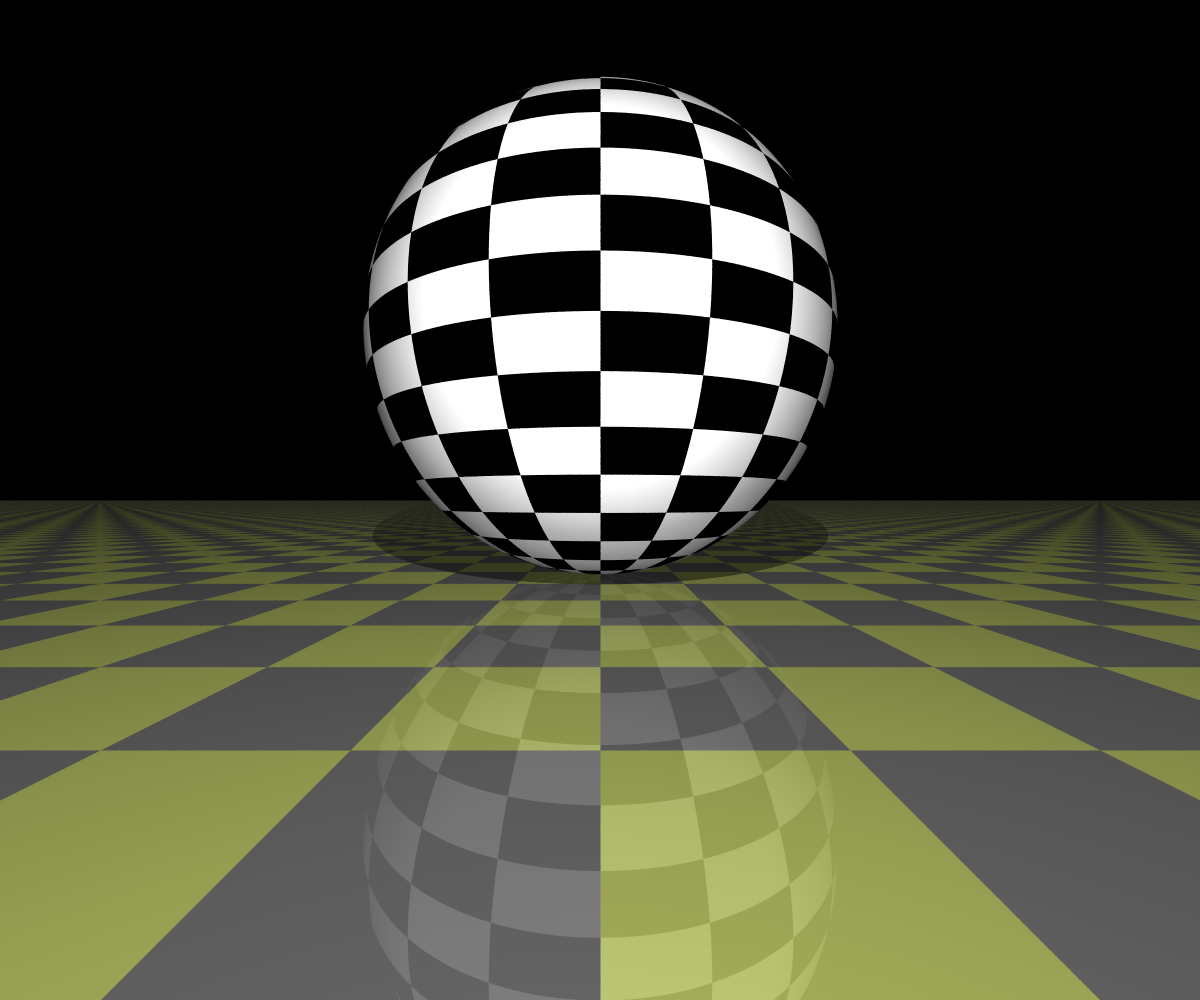
\includegraphics[width=\textwidth]{./examples/AntiAliasingComparison/Scene_random64.png}
    \caption{64x AA using random sampling.}
\end{figure}

\pagebreak

\begin{figure}[H]
    \centering
    \subfloat[Plane]{{ 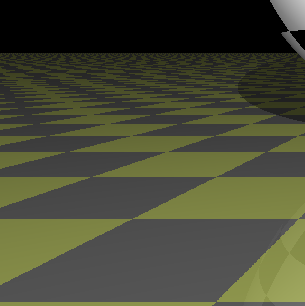
\includegraphics[width=0.3\textwidth]{./examples/AntiAliasingComparison/CheckeredPlane_noAntiAliasing.png} }}
    \subfloat[Sphere]{{ 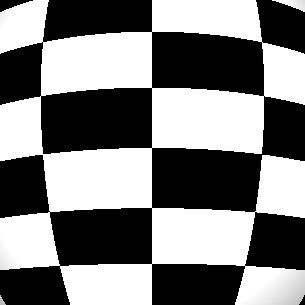
\includegraphics[width=0.3\textwidth]{./examples/AntiAliasingComparison/CheckeredSphereCrop_noAntiAliasing.png} }}
    \caption{Vanishing plane and checkered sphere without anti-aliasing.}
\end{figure}

\begin{figure}[H]
    \centering
    \subfloat[Plane]{{ 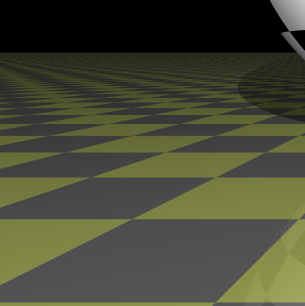
\includegraphics[width=0.3\textwidth]{./examples/AntiAliasingComparison/CheckeredPlane_regular64.png} }}
    \subfloat[Sphere]{{ 
\includegraphics[width=0.3\textwidth]{./examples/AntiAliasingComparison/CheckeredSphereCrop_regular64.png} }}
    \caption{Vanishing plane and checkered sphere with 64x AA using regular sampling.}
\end{figure}

\begin{figure}[H]
    \centering
    \subfloat[Plane]{{ 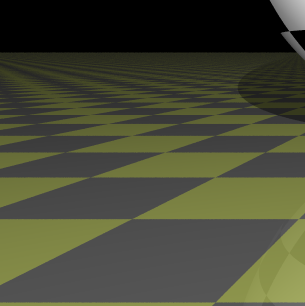
\includegraphics[width=0.3\textwidth]{./examples/AntiAliasingComparison/CheckeredPlane_random64.png} }}
    \subfloat[Sphere]{{ 
\includegraphics[width=0.3\textwidth]{./examples/AntiAliasingComparison/CheckeredSphereCrop_random64.png} }}
    \caption{Vanishing plane and checkered sphere with 64x AA using random sampling.}
\end{figure}

\end{document}
